\section{Simulation}
Simulations are conducted in the Gazebo simulator within the ROS environment. UAV used in experiments is the $\mu$Morus which can be found in the \textit{mmuav\_gazebo} repository \cite{gitLink}, along with its model parameters. Two experiments are conducted with UAVs using two different methods of CoG variation: MMC in the first case and payload carried by manipulators in the second case. \\
Control parameters for the first case are chosen as follows:
\begin{equation*}
	\text{k}_x = 
	\begin{bmatrix}
		10 &  0  &  0 \\
		 0 & 10  &	0 \\ 
		 0 &  0  & 50 	
	\end{bmatrix}
	\, , \,	
	\text{k}_v =
	\begin{bmatrix}
		3.75 & 0 & 0 \\
		0 & 3.75 & 0 \\
		0 & 0 & 20
	\end{bmatrix}
	\, , \,
\end{equation*}
\begin{equation*}
	\text{k}_R = 
	\begin{bmatrix}
		1.5 & 0 & 0 \\
		0 & 1.5 & 0 \\
		0 & 0 & 10
	\end{bmatrix}
	\, , \,
	\text{k}_\Omega = 
	\begin{bmatrix}
		0.65 & 0 & 0 \\
		0 & 0.65 & 0 \\
		0 & 0 & 1.54
	\end{bmatrix}
	\, , \,
\end{equation*}

\noindent Rotational control parameters, in the second case, stay the same, while translational parameters are the following: 
\begin{equation*}
	\text{k}_x = 
	\begin{bmatrix}
		7.2 &  0  &  0 \\
		0 & 7.2  &	0 \\ 
		0 &  0  & 50 	
	\end{bmatrix}
	\, , \,	
	\text{k}_v =
	\begin{bmatrix}
		2.6 & 0 & 0 \\
		0 & 2.6 & 0 \\
		0 & 0 & 20
	\end{bmatrix}
	\, , \,
\end{equation*}
For both cases, initial parameters are obtained by considering the error dynamics \eqref{error_dynamics_linear} and \eqref{error_dynamics_angular} in the equilibrium state. However, they are further tuned with better position tracking performance in mind.\\
It is important to note that the actuator dynamics of moving masses and manipulators is taken in consideration within the Gazebo simulator. Furthermore there is a slight transient delay while increasing or decreasing rotor velocity which results in a non-instantaneous control force change. \\
\indent The chosen trajectory tracking problem is formulated as a rotating spiral:
\begin{gather*}
	\textbf{x}_d(t) = [0.4\text{t}; \, 0.5\text{sin}(\pi\text{t}); \, 0.6\text{cos}(\pi\text{t}) + 2] \\
	\textbf{b}_{1,d}(t) = [\text{cos}\left(\frac{\pi}{5}\text{t}\right); \, \text{sin}\left(\frac{\pi}{5}\text{t}\right); \, 0]
\end{gather*}
\begin{figure}[h!]
	\centering
	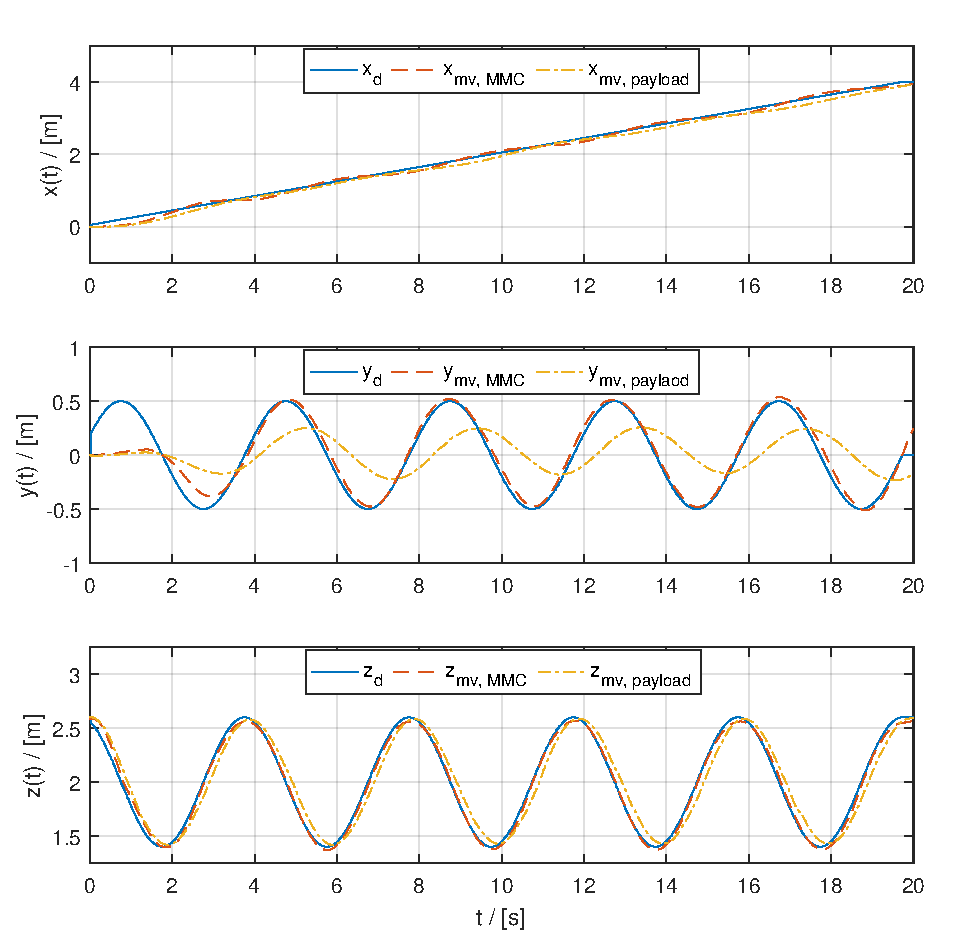
\includegraphics[width=\columnwidth]{./pictures/both_pos.pdf}
	\caption{Comparison between desired $\textbf{x}_d$ and measured position values $\textbf{x}_{mv}$ for both simulation cases. While tracking on x and z axes are reasonably similar, slower position tracking can be observed on the y axis for the second simulation case. Calculated MSE values are 0.0079 and 0.00352 for first and second case respectively.}
	\label{fig:traj_pos}
\end{figure}

\begin{figure}
	\centering
	\begin{minipage}{0.5\columnwidth}
		\centering
		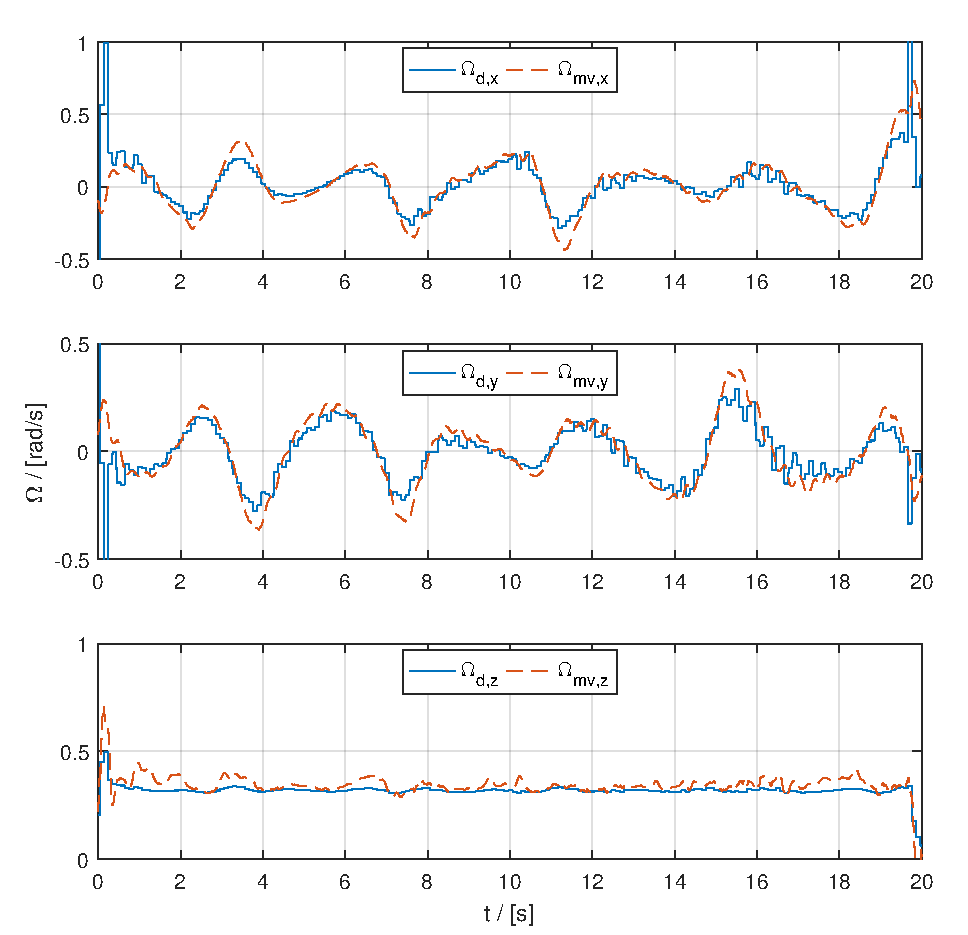
\includegraphics[width=\columnwidth]{./pictures/mmcuav_omega.pdf}
		\caption*{a) UAV with MMC}
		\label{fig:mmcuav_omega}
	\end{minipage}%
	\begin{minipage}{0.5\columnwidth}
		\centering
		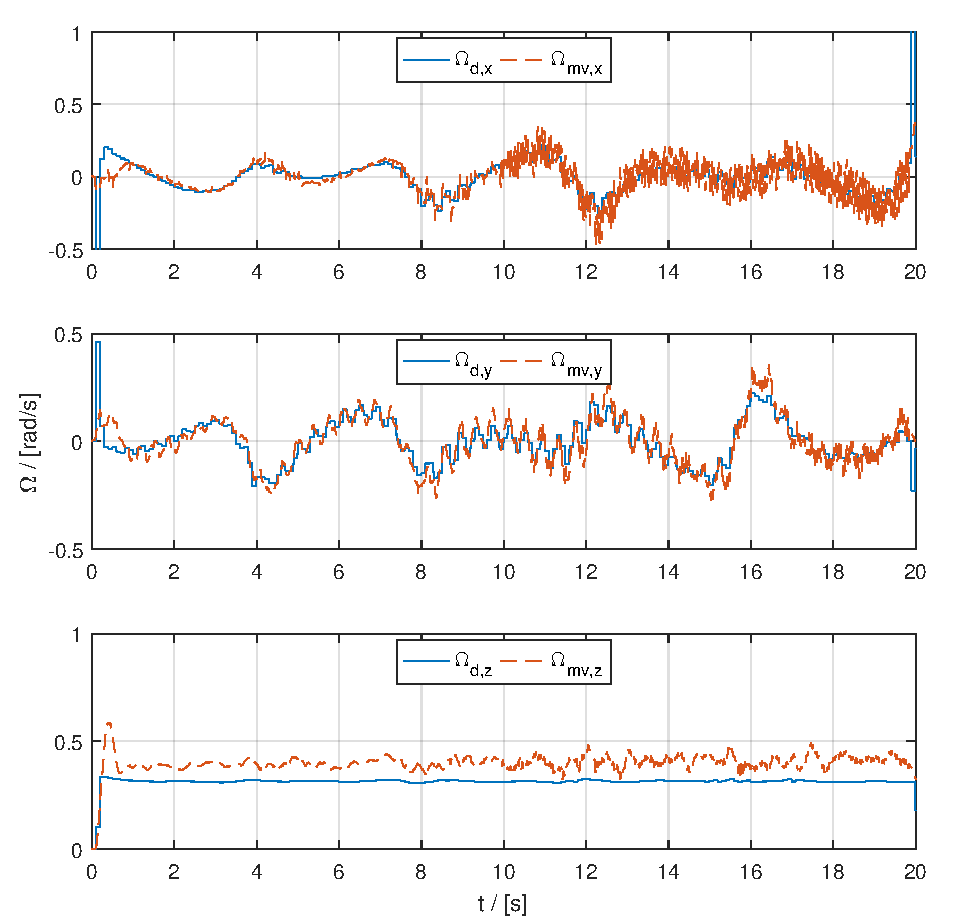
\includegraphics[width=\columnwidth]{./pictures/mmuav_omega.pdf}
		\caption*{b) UAV carrying a payload}
		\label{fig:mmuav_omega}
	\end{minipage}
	\caption{Comparison between desired $\mb{\Omega}_d$ and measured $\mb{\Omega}_{mv}$ angular velocities for both simulation cases. Better angular velocity tracking is achieved in the first case, while in the second case an oscillatory measured value is observed around x axis during later stages of trajectory tracking. It is interesting to note that although desired position and heading are the same for each case, a different desired angular velocity is obtained using \eqref{eqn:omega_d}.}
\end{figure}

\begin{figure}
	\centering
	\begin{minipage}{0.5\columnwidth}
		\centering
		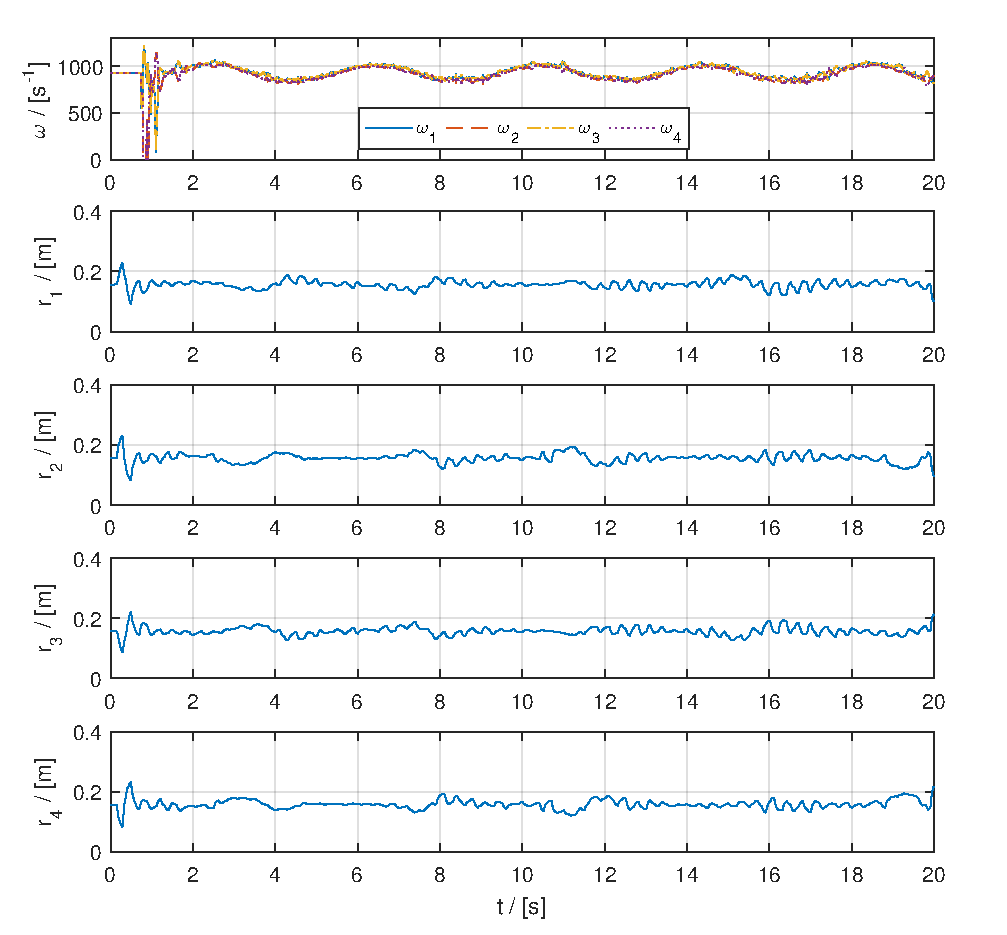
\includegraphics[width=\columnwidth]{./pictures/mmcuav_control_inputs.pdf}
		\caption*{a) UAV with MMC}
		\label{fig:mmcuav_control}
	\end{minipage}%
	\begin{minipage}{0.5\columnwidth}
		\centering
		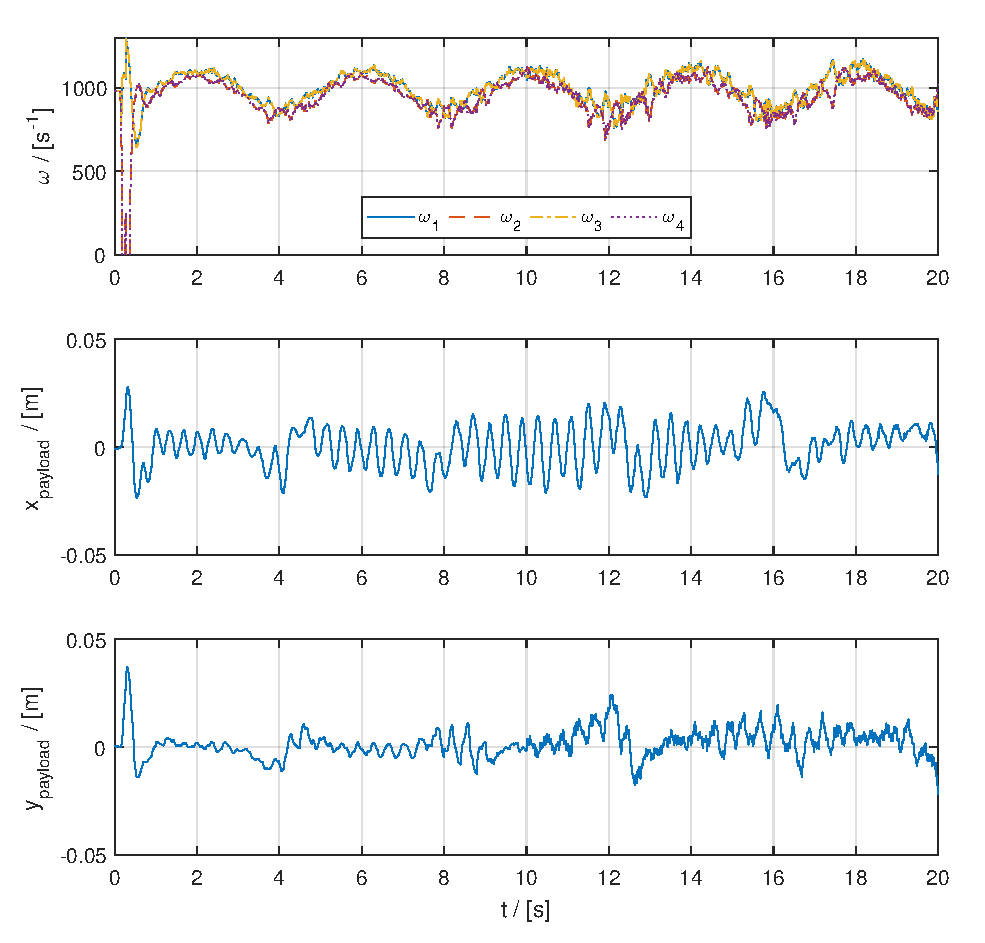
\includegraphics[width=\columnwidth]{./pictures/mmuav_control_inputs.pdf}
		\caption*{b) UAV carrying a payload}
		\label{fig:mmuav_control}
	\end{minipage}
	\caption{Figures show control inputs for both simulation cases: rotor velocities $\omega_i$, moving mass and payload offsets $r_i$. Rotor velocities are similar because desired trajectory height is equal for both cases.}
\end{figure}


\begin{figure}[h!]
	\centering
	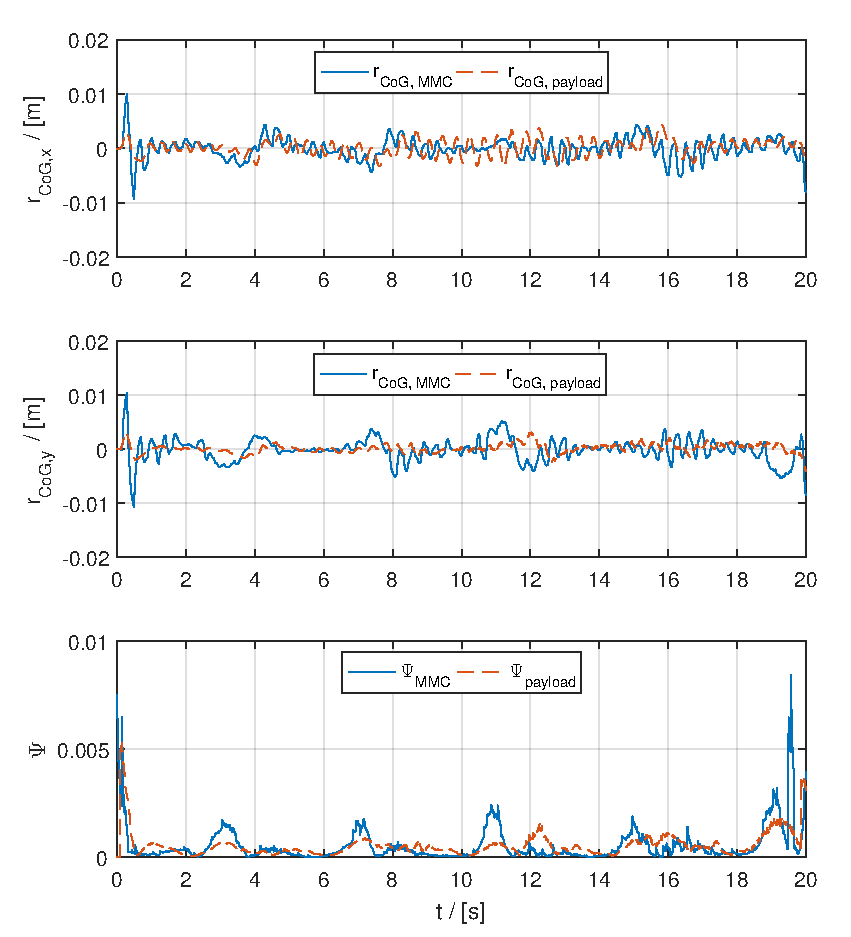
\includegraphics[width=\columnwidth]{./pictures/both_cog_err.pdf}
	\caption{Comparison between first two components of CoG vector $\textbf{r}_{CoG}$ and between attitude error functions $\Psi$ for both simulation cases. It can be seen that higher magnitude of CoG variation can be achieved using moving masses rather than the carried payload.}
	\label{fig:cog_error}
\end{figure}